\documentclass[11pt, a4paper, reqno]{scrartcl}

\usepackage[utf8]{inputenc}
\usepackage{a4wide}
\usepackage{libertine}
\usepackage{graphicx}
\usepackage{listings}
\usepackage{xcolor}
\usepackage{float}
\usepackage{amsmath}

% for latex output of pandas
\usepackage{booktabs}

\begin{document}
    \title{Exercise No. 2}
    \author{David Bubeck, Pascal Becht, Patrick Nisbl\`e}
    \maketitle
    
    \lstset{
        language=Python,
        backgroundcolor=\color{gray!10},
        numbers=left,
        captionpos=t,
        breaklines=true,
        frame=l,
        xleftmargin=\parindent,
        basicstyle=\footnotesize\sffamily,
        keywordstyle=\bfseries\color{green!40!black},
        commentstyle=\itshape\color{purple!40!black},
        identifierstyle=\color{blue!60!black},
        stringstyle=\color{orange}
    }

    \newpage
    \section*{2 - Error analysis of the Euler scheme}

    	\subsection*{a)}
			At first we write the code for the 2 - body problem by using the 
			forward Euler algorithm. We integrate the problem for one orbit and 
			plot it on a double - logarithmic scale. The error will be plotted 
			as a function of $\Delta t$. Therefore we will be using three 
			different eccentricities and various different time steps.
			\newline
			
			Function that integrates the 2 - body problem using the forward 
			Euler algorithm.
			
    		\begin{figure}[H]
        		\lstinputlisting[language=Python,
        			caption={Exercise02a.py},
        			lastline=27]{Exercise02a.py}        
    		\end{figure}
    		
    		
    		Now we plot a circular orbit with the error in energy in a 
    		additional plot. The values that were used are given in the code and We repeat the calculation for two more different initial velocities.
    		
    		\begin{figure}[H]
        		\lstinputlisting[
        			language=Python,
        			caption={Exercise02a.py},
        			firstnumber=30,
        			firstline=30]
        			{Exercise02a.py}   
    		\end{figure}
    		
    		\begin{figure}[H]
    			\centering
    			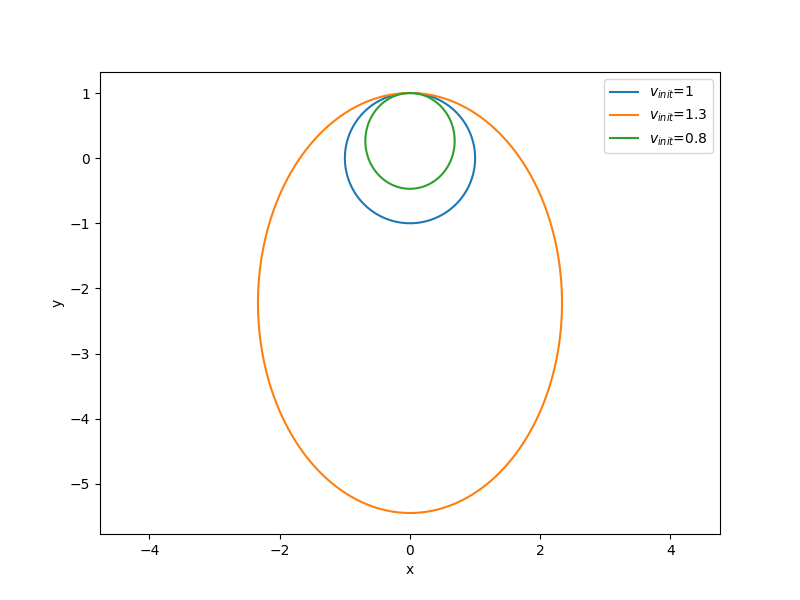
\includegraphics[height=.33\paperheight]{fig_a1.png}
    			\caption{First orbit with forward Euler algorithm}
    		\end{figure}
    		
    		\begin{figure}[H]
    			\centering
    			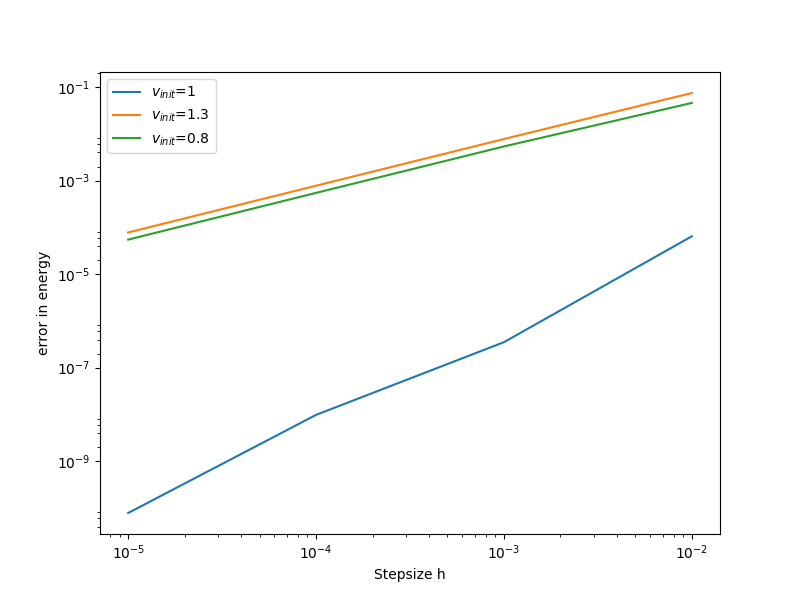
\includegraphics[height=.33\paperheight]{fig_a2.png}
    			\caption{First orbit energy error with forward Euler algorithm}
    		\end{figure}
    		
    		
    		
    		
    	\newpage
    		
    	\subsection*{b)}
			Now we write the code for the 2 - body problem by using the 
			Leapfrog algorithm. We integrate the problem for one orbit and 
			plot it on a double - logarithmic scale. The error will be plotted 
			as a function of $\Delta t$. Therefore we will be using three 
			different eccentricities and various different time steps.
			\newline
			
			Function that integrates the 2 - body problem using the Leapfrog 
			algorithm.
			
    		\begin{figure}[H]
        		\lstinputlisting[language=Python,
        			caption={Exercise02b.py},
        			lastline=31]{Exercise02b.py}        
    		\end{figure}
    		
    		
    		Now we plot a circular orbit with the error in energy in a 
    		additional plot. The values that were used are given in the code. To be precise we going to use the same values as before and we also repeat the calculation for two more different initial velocities.
    		
    		\begin{figure}[H]
        		\lstinputlisting[
        			language=Python,
        			caption={Exercise02b.py},
        			firstnumber=34, 
        			firstline=34
        		]{Exercise02b.py}   
    		\end{figure}
    		
    		\begin{figure}[H]
    			\centering
    			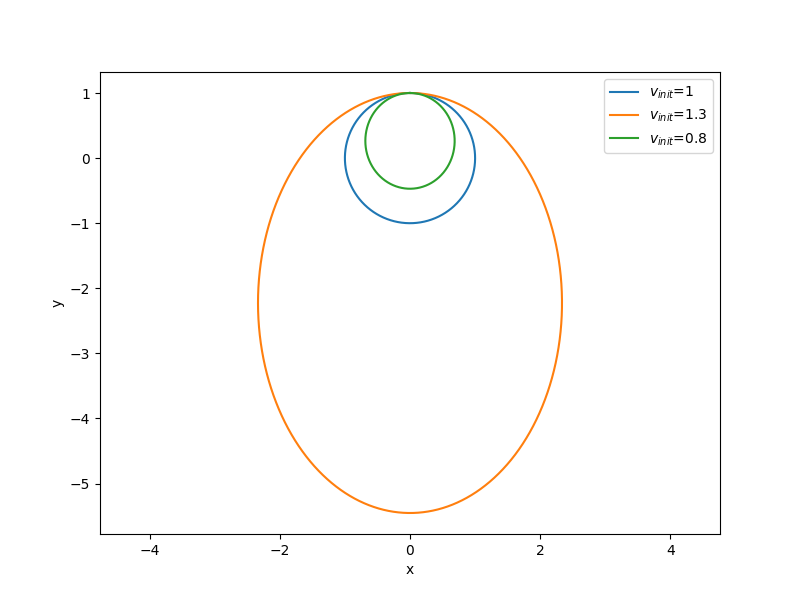
\includegraphics[height=.33\paperheight]{fig_b1.png}
    			\caption{First orbit with leapfrog algorithm}
    		\end{figure}
    		
    		\begin{figure}[H]
    			\centering
    			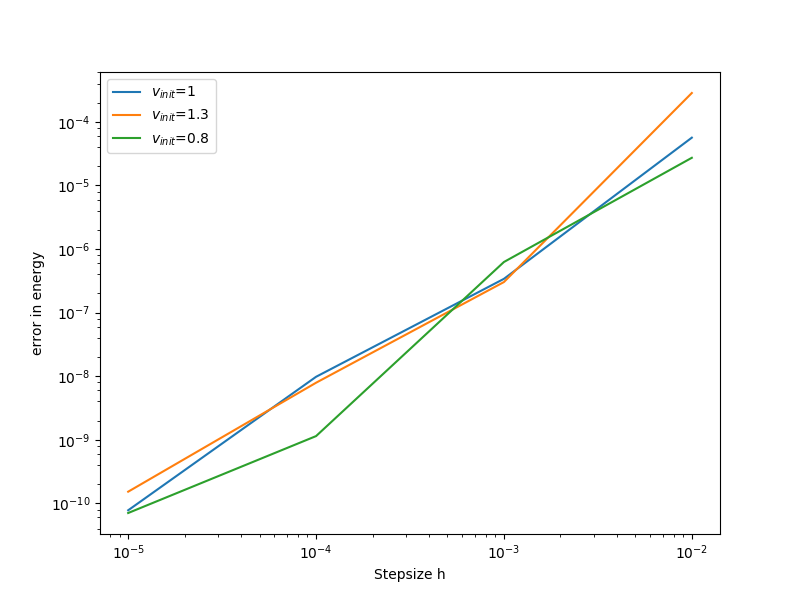
\includegraphics[height=.33\paperheight]{fig_b2.png}
    			\caption{First orbit energy error with leapfrog algorithm}
    		\end{figure}
    		
    		The errors decrease with decreasing time steps for both integration 
    		schemes. For the Euler algorithm we expect a drop with $O(h^2)
    		$, for the Leapfrog algorithm $O(h^3)$. This is also what we can observe. The errors of the Leapfrog integration are much smaller than those of the Euler integration. However, the slope of the error-curve is 
    		steeper which we also expected. Another difference between the error-plots, of the two integration variants is, that for the Euler integration we get straight lines whereas for the Leapfrog integration the errors seem to scatter around the expected line. 

\end{document}